\chapter{做问卷调查} % Introduction chapter suppressed from the table of contents

要做好数据分析,便要制定计划 - 收集那些数据,如何收集,如何存储数据,
准备后面如何分析数据。

思路类似如何设计问卷调查,先看以下案例。

\hypertarget{ux6848ux4f8bux4e3aux67d0ux5168ux56fdux5febux9910ux8fdeux9501ux505aux95eeux5377ux8c03ux67e5}{%
\subsection{案例:为某全国快餐连锁做问卷调查}\label{ux6848ux4f8bux4e3aux67d0ux5168ux56fdux5febux9910ux8fdeux9501ux505aux95eeux5377ux8c03ux67e5}}

美国一家连锁快餐店,全国有三万员工。但员工流失率严重(接近百分百)。人事部估计聘用、培训、建档案等,每个新员工要花费三百美金成本。粗略估计每年由于员工流失就产生一千万美金的成本,差不多是整个集团的盈利。\\
虽然高层一直知道,但觉得大量员工流失率是快餐业的通病,所以没有注意。咨询顾问针对这问题,详细查看流失率的分布,发现不同店铺的员工流失率差异很大
- 从最低6\%到最高 800\%。\\
%===详细分析===
\hypertarget{ux4eceux5206ux6790ux5230ux884cux52a8}{%
\subsubsection{详细分析}\label{ux4eceux5206ux6790ux5230ux884cux52a8}}
抽看其中一百家餐厅,把每年流失率在120\%以上的当成高,60\%以下的当成低,分析数据发现在各种职位:前厅、后厨、维修工人等。发现员工流失率与工种无关,主要是跟餐厅有关。\\
%===研究高流失率的原因===

\hypertarget{ux4eceux5206ux6790ux5230ux884cux52a8}{%
\subsubsection{研究高流失率的原因}\label{ux4eceux5206ux6790ux5230ux884cux52a8}}

\begin{itemize}
\tightlist
\item
  随机抽样10家餐厅,4家属于每年流失率40\%到60\%之间,2家是中等水平(60\%到120\%之间),4家属于高等
  (每年超过120\%)
\item
  做问卷调查,有39条问题
\item
  初步分析发现高与低流失率被抽样单位,发现它们的员工的年龄;被餐厅聘用了多少年;工种;是否轮班;等分布都很类似,所以这些都不是原因。
\item
  主要原因是在管理者的态度。比如,低流失率餐厅的员工,在39条问题里,关于管理层的31条都比高流失率餐厅员工较高分。
\item
  低流失率餐厅的员工觉得他们得到较好的辅导,经理比较乐意帮助他们,甚至更有机会升职。
\item
  低流失率餐厅的员工更满意工作和薪酬(其实无论高与低流失率餐厅的工资水平大致一样)
\item
  下图是9条最有代表性的问卷结果:
\end{itemize}

%\href{文件:WeisbordP218.2.jpg}{thumb\textbar{}none\textbar{}500px\textbar{}图1}\\

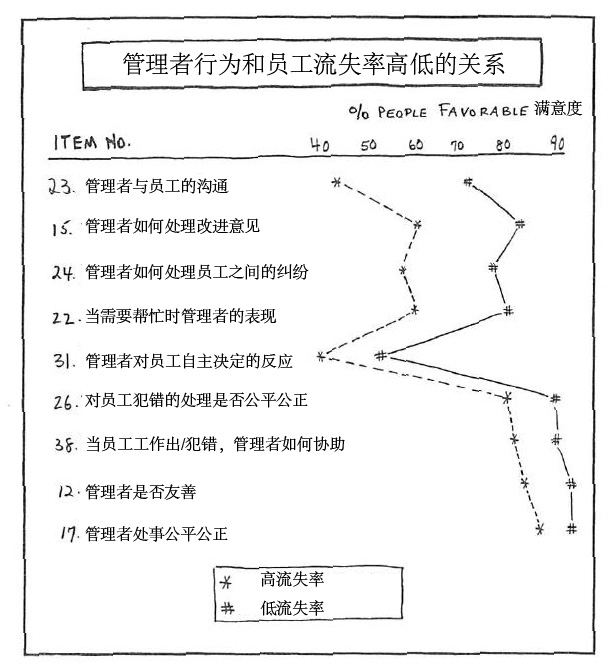
\includegraphics[width=6cm]{WeisbordP2182.jpg}

\hypertarget{ux4eceux5206ux6790ux5230ux884cux52a8}{%
\subsubsection{从分析到行动}\label{ux4eceux5206ux6790ux5230ux884cux52a8}}

把那些关于管理者的态度如何影响餐厅员工流失率总结成下图,让管理层更了解主因:\\
%\href{文件:WeisbordP219.1.jpg}{thumb\textbar{}none\textbar{}500px\textbar{}图2}\\

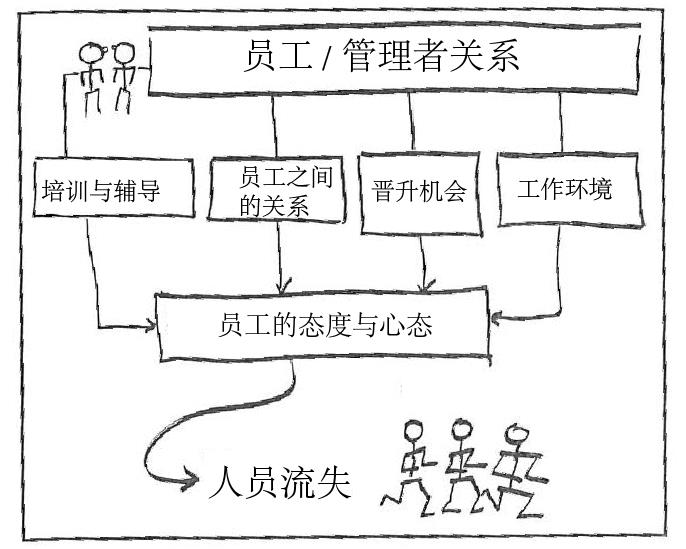
\includegraphics[width=6cm]{WeisbordP2191.jpg}

因为经理与员工的关系影响到培训、员工的成长机会、晋升的机会、员工之间的关系等,直接影响到员工流失。

\hypertarget{ux9488ux5bf9ux53d1ux73b0ux5f00ux59cbux505aux5b9eux9a8c}{%
\subsubsection{针对发现开始做实验}\label{ux9488ux5bf9ux53d1ux73b0ux5f00ux59cbux505aux5b9eux9a8c}}

为某区域的餐厅经理做针对性培训,也让他们看到从问卷调查,他们店的成绩与全国其他餐厅的比较。在四天培训里面,我们针对问题解决、领导能力等做针对性培训。这些培训不仅仅是老师讲课那种,大部分是利用角色扮演,首先列出来他们希望新员工要学到哪些点,然后用角色扮演,在那个新员工的入职培训里面如何执行,自己评判效果或者表现如何。他们也跟高层经理交流,可以反映一些他们在自己餐厅单独解决不了的问题。

\hypertarget{ux6bd4ux8f83ux57f9ux8badux540eux6548ux679c}{%
\subsubsection{比较培训后效果}\label{ux6bd4ux8f83ux57f9ux8badux540eux6548ux679c}}

\begin{itemize}
\tightlist
\item
  发现在27个餐厅中,参加过培训的24家后期员工流失率显著降低。例如其中一家有29位员工,以前是一年走了37位,但做了培训后,没有流失。整个做实验的区平均下来,流失率减少了50\%。\\
\end{itemize}

从以上案例可以看到依据目标制定一些度量项------就是问哪些问题。之前也有一些基本的分析,比如以什么维度去分析,比如前面发现跟工种无关,主要是针对不同餐厅,问卷调查也验证了本来那个猜测,这是经理跟员工之间的关系影响到流失。问卷调查证明了这个关系后,就有对应的改进措施。措施实施后,效果是否有显著的完善。

从以上案例,看到如何针对改进的目标,设计问卷,收集数据,利用数据分析帮助找出根本原因,
制定针对根因的改进措施,然后评判改进效果。

%\href{文件:tys51_1.0.png}{500px}

\includegraphics[width=6cm]{tys51_10.png}

看上图 ,度量计划应包括:

\textbf{度量目标} - 为何要度量,要解答什么问题\\
\textbf{度量项} - 收集什么度量 (对什么对象,问什么问题)\\
\textbf{收集数据, 分析数据} -
用什么形式来度量,如何分析,这个是在度量前要想好,有些很重要的因素忘记问,后面无法补。所以我们度量与分析也是这个思路。

\hypertarget{ux603bux7ed3}{%
\subsection{总结}\label{ux603bux7ed3}}

度量分析的计划都应该包含下面要素:\\
1) \textbf{明确度量目标}
希望改进什么?然后依据目标或者预估影响结果的可能因素。例如,是否跟管理者的领导和沟通能力相关。然后依据这思路,制定问卷内容。

2) \textbf{度量项的操作定义}
如果定义不清楚,可能不同团队因为理解不一样,提供的数据就不同了。

\begin{itemize}
\tightlist
\item
  如何确保数据的质量。因为如果数据本身不对,后面什么分析都没用。如果有系统记录,可以利用系统验证数据是否正确。但反过来,如果是数据都是凭经理在项目结束最后填一个表给你的话,就会怀疑这些数字有多少的可信度。
\end{itemize}

3) \textbf{数据怎么获取}
尤其是在软件开发。如果他们没有记录缺陷或者工时,很多数据就无法在回顾时获得,没有数据就没法做后面的分析。然后在做计划时,要想假如那些数据收集到之后要怎么分析?例如,如果问卷没有收集一些餐厅的基本数据,比如区域、员工数量、入职时长等基本数据,后面就无法用这些维度去分析。

4) \textbf{数据存储}
为了方便后面的统计分析,应该形成一个数据表的格式,比如是一行是一个项目或一个迭代,每一列就是不同的变量,方便后面累加数据,可以不用修改就直接分析了。






